\chapter{Utilizing Onboard Compute In SteelEagle}

This chapter discusses work to replace the communications relay used in
SteelEagle to the Modal AI VOXL 2. The VOXL 2 offers significant computational
capability, allowing the execution of Tensorflow Lite machine learning models.
We start by characterizing this shift in offloading strategy in more general
terms.

\section{The Computation Offload Spectrum}
\begin{figure}[htbp]
\centerline{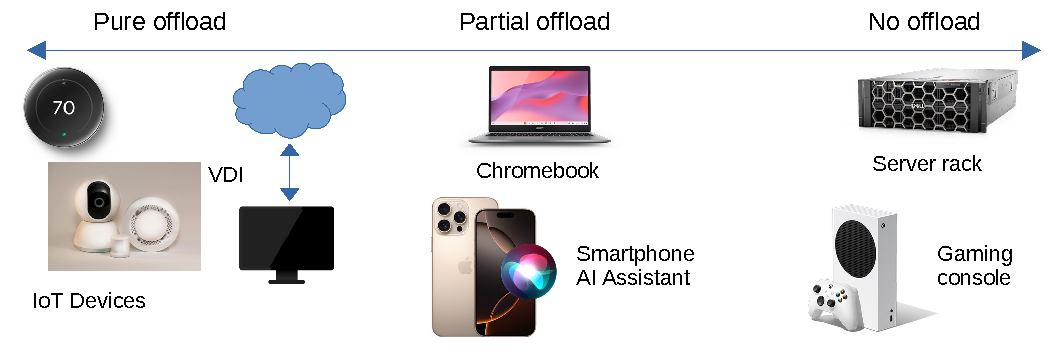
\includegraphics[width = .8\textwidth]{figs/offload-spectrum-crop.pdf}}
\caption{Devices Placed in the Computation Offloading Spectrum}
\label{fig:offload-spectrum}
\end{figure}
Devices today leverage offloading to various degrees.
\Cref{fig:offload-spectrum} shows how devices can be placed in an offloading
spectrum, with thin clients found towards the left of the spectrum and thick
clients to the right. A thin client, as opposed to a thick client, has minimal
compute and can be made smaller, lighter, and cheaper. Virtual desktop
infrastructure (VDI), for example, leverages pure offload by providing remote
access to desktops hosted on centralized servers.  This reduces the
computational demands on the client device, enabling the use of
computationally-intensive applications on weaker and older ``thin'' hardware,
reducing costs. Similarly, internet-of-things (IoT) sensors, such as video
cameras, cirumvent their limited storage and computational ability by
leveraging pure offload, transmitting their sensor streams to the cloud for
storage and analysis.

On the other end of the spectrum, we find devices such as gaming consoles,
desktop computers, and autonomous cars. Gaming consoles and desktop computers
are expected to have crisp interaction, which is not achievable by offloading
to cloud. Offloading to cloudlets, which can provide low latency, is not a
feasible option for these devices currently because of the absence of
widespread cloudlet infrastructure.  Gaming consoles and desktop computers can
provide high-levels of onboard computational power because they are not subject
to mobility constraints.  Although autonomous cars are mobile, they typically
have sufficient energy available to perform intensive onboard computations
since the majority of energy is needed to propel the car forward. They must
also perform real-time decision making reliably even in the absence of network
connectivity, which makes offloading less appealing.

In the middle of the spectrum, we find devices that perform partial offloading.
These devices have sufficient computational power to function when offloading
is unavailable or not advantageous, but they also offload computation in other
cases. Smartphone AI voice assistants such as Apple's Siri, for example,
originally offloaded all computation to the cloud. Over time, it evolved to
utilize on-device capabilities to perform simpler tasks, allowing its use in
the absence of an internet connection.  Chromebooks were designed with a focus
on the use of cloud-based services, allowing them to be fitted with lower
processing power, memory, and storage capacity compared to traditional laptops.

\subsection{How should applications decide the offloading strategy?}
\label{sec:deciding-offloading-strategy}

Choosing an offload strategy for a given application can be done based on some
key attributes that are considered important for the application:
\begin{enumerate}
    \item \textbf{Mobility requirements}: is the application subject to
        mobility constraints?
    \item \textbf{Disconnected operation}: does the application need to work reliably
        in the face of network disconnection or degradation? Is degraded operation
        acceptable during disconnected operation?
    \item \textbf{Latency requirements}: is the application latency-sensitive?
        Are there tasks that are computationally intensive but can tolerate
        high latency if a nearby cloudlet is unavailable?
    \item \textbf{Bandwidth constraints}: how much network bandwidth is
        available to the application?
    \item \textbf{Cost requirements}: is low cost for devices a priority in
        this application?
\end{enumerate}

These attributes encapsulate the benefits and limitations of offloading.
Offloading is typically only relevant for mobile devices. A mobile device that
is dependent entirely on offloading will be unable to function adequately when
offloading is impossible altogether because of network disconnection, or
impacted because of degraded network conditions, such as high latency and low
bandwidth availability. Applications that are mission-critical would be wise to
equip devices with sufficient computational resources to support an acceptable
level of function when adverse network conditions impact offloading.
Applications that are not mission-critical can rely on pure offload to benefit
from the cost savings resulting from using devices that are not required to
have significant computational resources.

Offloading allows mobile devices to achieve a much higher level of
functionality that their onboard hardware allows for. Equipping mobile devices
with the hardware needed to maintain the same level of functionality during
offload degradations reduces the benefit of offloading---the mobile device is
weighed down with the additional size and weight of more complex hardware that
remains unused when offloading is possible.

If offload degradations are infrequent, a more reasonable approach is to
utilize the inferior on-device computational resources to compute results that
are inferior according to an output-specific metric, compared to those obtained
using offloading. For predictions from a machine learning model, the metric
could be the accuracy of the prediction. In previous work, the concept of
\textit{fidelity} has been used in this context, defined as the degree to which
the results differ according to the metric \cite{noble1997}.

\subsection{The dynamic nature of partial offload}

Network conditions affect the performance of offloading, but they are dynamic
in nature. Mobile devices utilizing partial offload, then, must decide an
offloading strategy at runtime. But the decision is not binary---exclusively
using onboard compute or remote compute resources.  As
\cref{fig:offload-spectrum} shows, there is a wide range between the two ends
of the spectrum. Depending on the current network conditions, partial-offload
mobile devices can utilize a combination of onboard and remote computational
resources that results in optimal performance.

Mobile devices can achieve this through an optimal partitioning of applications
into local and remote components. Flinn et al tackled the issue of developing
applications that can support devices with different capabilities and dynamic
execution conditions with a self-tuning remote execution system. The system,
called \textit{Spectra}, continuously monitors the application's resource
supply and demand and suggests which components of an application should be
executed remotely, taking into account factors such as performance, energy
usage, and fidelity \cite{flinn2002}. This work requires the application
developer to partition the application, specifying application components
that could benefit from remote execution.

\subsection{Offloading shaping}
\label{sec:offload-shaping}

Hu et al \cite{hu2015} showed that there is value to doing additional onboard
computation when offloading, which was not originally part of the application.
The approach, called \textit{offload shaping}, attempts to conserve wireless
bandwidth and energy through the process of \textit{early discard}. The process
involves selectively sending inputs for offload computation based on an
application-specific metric of value assigned to each input.  In the case of
video analytics, for instance, onboard computation can detect blurry frames and
not transmit them to the cloudlet. Hu et al showed that object recognition does
not perform well on blurry frames, and so it is a waste of bandwidth and energy
to transmit these blurry frames to a cloudlet for computation.

\section{A Partial Offload Pipeline for SteelEagle}

SteelEagle drones can currently be placed in the ``pure offload'' part of the
spectrum in \cref{fig:offload-spectrum}, since they do not perform any on-board
computation other than the encoding of the raw camera feed to an RTSP H.264
video stream that is transmitted to a cloudlet. As discussed in
\cref{sec:deciding-offloading-strategy}, a pure offload strategy does not
support disconnected operation, and impacts the application considerably as
network conditions degrade.

\begin{figure}[htbp]
\centerline{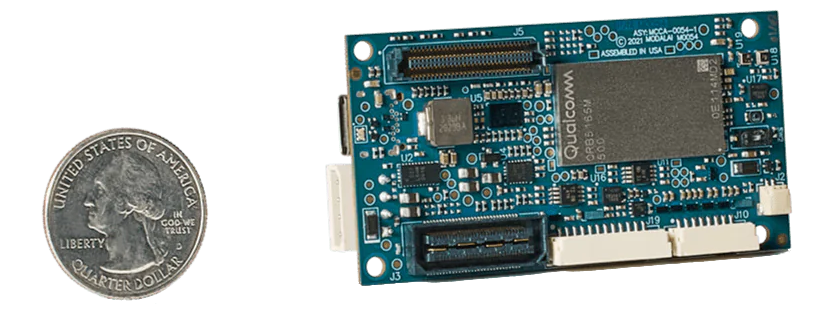
\includegraphics[width = .5\textwidth]{figs/voxl2.png}}
\caption{Modal AI VOXL 2}
\label{fig:voxl2}
\end{figure}

Replacing the Onion Omega 2 with the Modal AI VOXL 2 (\cref{fig:voxl2}) as the
communications relay in the SteelEagle pipeline will allow us to pursue a
partial offloading strategy that allows SteelEagle drones to gracefully react
to changes in network conditions. Intended for use as an AI autopilot in custom
drones, the VOXL 2 features a Qualcomm QRB5165 processor and a PX4 flight
controller. We do not utilize the PX4 flight controller on the VOXL.
\Cref{tab:voxl2-specs} provides information about the computational resources
available on the VOXL 2.

\begin{table}[htbp]
    \centering
    \begin{tabular}{@{}ll@{}}
        \toprule
        \textbf{} & \textbf{ModalAI VOXL 2}\\
        \midrule
        \textbf{Architecture} & 64-bit ARM\\
        \textbf{CPU} & Qualcomm Kyro 585 (7nm, released Dec 2019)\\
                     & 1 x 2.84 GHz high-performance core\\
                     & 3 x 2.42 GHz high performance cores\\
                     & 4 x 1.80 GHz low-performance cores\\
        \textbf{ISP} & Qualcomm Spectra 480\\
        \textbf{GPU} & Qualcomm Adreno 650, with support for OpenCL\\
        \textbf{DSP} & Qualcomm Hexagon 698\\
        \textbf{Memory} & 8 GB\\
        \textbf{Weight} & 16 grams\\
        \textbf{Power consumption} & 4-5 W under high load\\
        \textbf{Operating system} & Ubuntu 18.04\\
        \bottomrule
    \end{tabular}
    \caption{The specifications of the QRB5165 processor used in the VOXL 2}
    \label{tab:voxl2-specs}
\end{table}

\begin{figure}[htbp]
\definecolor{observe-color}{RGB}{175,208,149}
\definecolor{orient-color}{RGB}{255, 255, 166}
\definecolor{decide-color}{RGB}{255,170,149}
\definecolor{act-color}{RGB}{224,194,205}
\centering
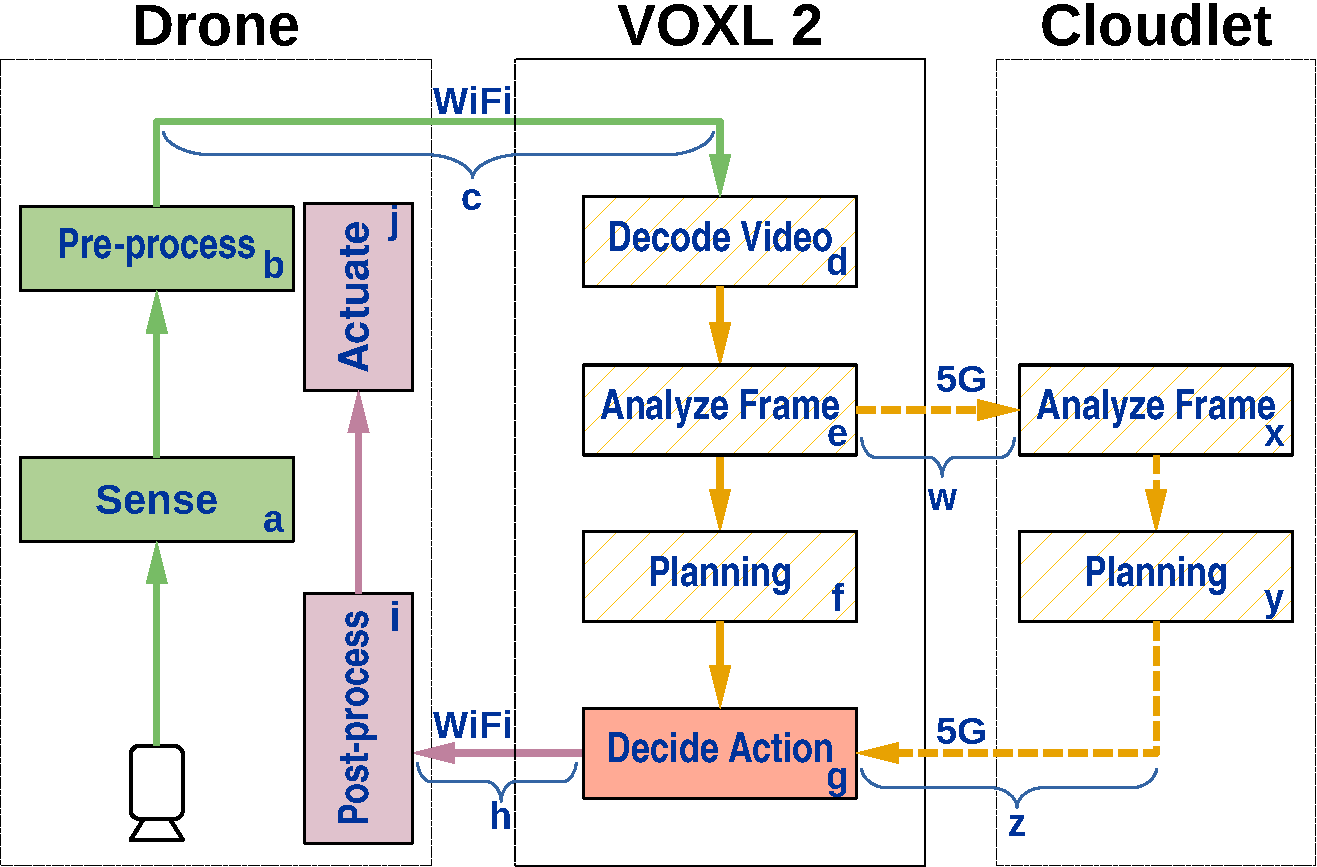
\includegraphics[width = .7\textwidth]{figs/fig-voxl-ooda-loop-crop.pdf}
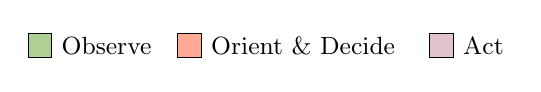
\begin{tikzpicture}
    \draw[fill=observe-color] (1.0,0) rectangle (1.3,0.3);
    \node[right] at (1.3,0.15) {\small Observe};

    \draw[fill=decide-color] (2.9,0) rectangle (3.2,0.3);
    \node[right] at (3.2,0.15) {\small Orient \& Decide};

    \draw[fill=act-color] (6.1,0) rectangle (6.4,0.3);
    \node[right] at (6.4,0.15) {\small Act};
\end{tikzpicture}
\caption{Mapping the VOXL 2 pipeline to the OODA loop}
\label{fig:voxl2-ooda-loop-mapping}
\end{figure}

The VOXL 2 has support for running Google's Lite Runtime (LiteRT) machine
learning models, formely known as TensorFlow Lite (TFLite). Trained TensorFlow
and PyTorch models can be converted to LiteRT models by using techniques such
as quantization and pruning \cite{jacob2017}. Float16 quantization reduces the
floating-point precision of the model's weights to 16-bits, and full integer
quantization converts them to integers. This reduces the model's size, memory
usage and inference latency, making it more suitable for mobile device
inferencing. Float16 quantization, for instance, reduces the size of the model
by half and causes minimal loss in accuracy. However, GPU acceleration of
float16-quantized models requires half-precision floating point support (FP16)
\cite{ho2017}.

\Cref{fig:voxl2-ooda-loop-mapping} depicts the new pipeline with the VOXL 2.
In the existing SteelEagle architecture, as described in
\cref{sec:steeleagle-bg}, video decoding is performed on the cloudlet since all
video stream network packets are forwarded to the cloudlet using the Onion
Omega as a network gateway. To perform onboard computation on the VOXL 2, we
must obtain individual frames from the drone's video stream.  This requires
decoding the H.264 video stream on the VOXL 2. As frames are decoded, the
pipeline can leverage offload shaping techniques (\cref{sec:offload-shaping})
to determine if the frame should be discarded. Then, a remote execution system,
such as the one developed by Flinn et al \cite{flinn2002}, can determine if
processing should be offloaded. Once frame processing is complete, the pipeline
determines whether any drone actuation needs to be performed, and generates the
corresponding command.

\subsection{Latency of VOXL 2 Onboard Pipeline}

\subsubsection*{Observe}

The Observe component of the OODA loop in the new pipeline retains on-drone
sensing and pre-processing, which involves generation of an RTSP H.264 video
stream from the drone camera's raw video frames. The video stream is
transmitted to the VOXL 2 over Wi-Fi, and is decoded.
\Cref{fig:voxl2-decoding-performance} shows the latency measurements. The
latency distribution has a mean of 262 ms, with a standard deviation of 10.5 ms
and a p99 of 282 ms. This is comparable to the Observe$_{ab}$ measurements from
the Onion Omega pipeline.

\subsubsection*{Orient \& Decide}

Orient involves performing inference on each frame to achieve the drone's
desired functionality. In our measurements we use the YOLOv5 model which is
used for detecting objects. \Cref{fig:voxl2-inference-hist} shows the latency
measurements.  The latency distribution has a mean of 60.5 ms and a p99 of 77.5
ms. The Decide component involves determining drone actuation and generation of
the drone command using the drone API, which is negligible.

\subsection*{Act}

In the onboard pipeline, as before, the Act component is measured as the time
taken for the drone's gimbal to start actuating after a command is issued from
the VOXL 2. In the case of the VOXL 2 pipeline, it requires a network hop over
the Wi-Fi segment from the VOXL 2 to the drone, post-processing on the drone to
process the command and electromechanical actuation of the drone's gimbal.
Figure xx

\begin{figure}[tbp]
\begin{minipage}[t]{0.45\textwidth}
\centerline{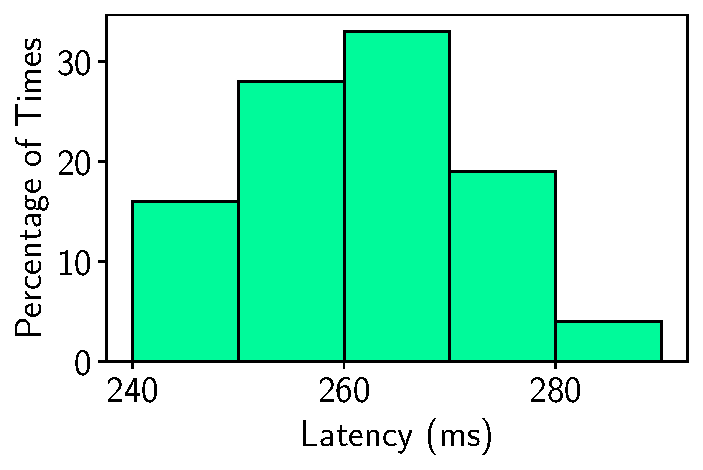
\includegraphics[width = \textwidth]{figs/onboard-decoding.pdf}}
\centering
Mean: 262$\pm$10.5~ms\; p99: 282~ms\\
\caption{Onboard H.264 video decoding performance on the VOXL 2}
\label{fig:voxl2-decoding-performance}
\end{minipage}
\hfill
\begin{minipage}[t]{0.45\textwidth}
\centerline{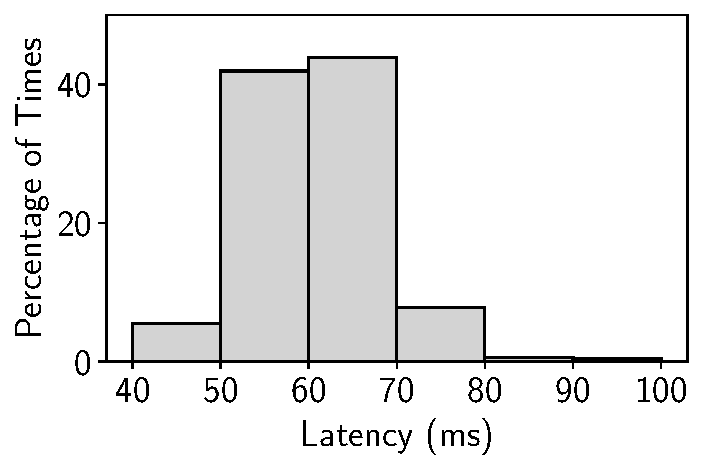
\includegraphics[width = \textwidth]{figs/onboard-inference-hist.pdf}}
\centering
Mean: 60.5$\pm$6.77~ms\; p99: 77.5~ms\\
\caption{Onboard inference on the VOXL 2 using a float16-quantized yolov5 model}
\label{fig:voxl2-inference-hist}
\end{minipage}
\end{figure}
